% Options for packages loaded elsewhere
\PassOptionsToPackage{unicode}{hyperref}
\PassOptionsToPackage{hyphens}{url}
%
\documentclass[
]{article}
\usepackage{amsmath,amssymb}
\usepackage{iftex}
\ifPDFTeX
  \usepackage[T1]{fontenc}
  \usepackage[utf8]{inputenc}
  \usepackage{textcomp} % provide euro and other symbols
\else % if luatex or xetex
  \usepackage{unicode-math} % this also loads fontspec
  \defaultfontfeatures{Scale=MatchLowercase}
  \defaultfontfeatures[\rmfamily]{Ligatures=TeX,Scale=1}
\fi
\usepackage{lmodern}
\ifPDFTeX\else
  % xetex/luatex font selection
\fi
% Use upquote if available, for straight quotes in verbatim environments
\IfFileExists{upquote.sty}{\usepackage{upquote}}{}
\IfFileExists{microtype.sty}{% use microtype if available
  \usepackage[]{microtype}
  \UseMicrotypeSet[protrusion]{basicmath} % disable protrusion for tt fonts
}{}
\makeatletter
\@ifundefined{KOMAClassName}{% if non-KOMA class
  \IfFileExists{parskip.sty}{%
    \usepackage{parskip}
  }{% else
    \setlength{\parindent}{0pt}
    \setlength{\parskip}{6pt plus 2pt minus 1pt}}
}{% if KOMA class
  \KOMAoptions{parskip=half}}
\makeatother
\usepackage{xcolor}
\usepackage{graphicx}
\makeatletter
\def\maxwidth{\ifdim\Gin@nat@width>\linewidth\linewidth\else\Gin@nat@width\fi}
\def\maxheight{\ifdim\Gin@nat@height>\textheight\textheight\else\Gin@nat@height\fi}
\makeatother
% Scale images if necessary, so that they will not overflow the page
% margins by default, and it is still possible to overwrite the defaults
% using explicit options in \includegraphics[width, height, ...]{}
\setkeys{Gin}{width=\maxwidth,height=\maxheight,keepaspectratio}
% Set default figure placement to htbp
\makeatletter
\def\fps@figure{htbp}
\makeatother
\setlength{\emergencystretch}{3em} % prevent overfull lines
\providecommand{\tightlist}{%
  \setlength{\itemsep}{0pt}\setlength{\parskip}{0pt}}
\setcounter{secnumdepth}{-\maxdimen} % remove section numbering
\ifLuaTeX
  \usepackage{selnolig}  % disable illegal ligatures
\fi
\IfFileExists{bookmark.sty}{\usepackage{bookmark}}{\usepackage{hyperref}}
\IfFileExists{xurl.sty}{\usepackage{xurl}}{} % add URL line breaks if available
\urlstyle{same}
\hypersetup{
  hidelinks,
  pdfcreator={LaTeX via pandoc}}

\author{}
\date{}

\begin{document}

Submission By

DA24C021 - Venkatesh Duraiarasan

CS24M033 - Pradeep Peter Murmu

\tableofcontents

\section{Assignment 1: Ontology
Design}\label{assignment-1-ontology-design}

\subsection{Task - 1}\label{task---1}

\subsubsection{\texorpdfstring{Domain of Interest
}{Domain of Interest }}\label{domain-of-interest}

The domain of interest is \textbf{financial instruments} from the
perspective of \textbf{retail investors}. The ontology aims to model the
sentiment associated with various financial instruments, such as stocks,
bonds, mutual funds, etc., based on information that retail investors
encounter (news headlines, snippets from annual reports, etc.). This
information includes company performance, market conditions, and
specific aspects of the company\textquotesingle s operations or
financial health. The goal is to automatically classify financial
instruments into either Positive or Negative categories based on the
sentiment derived from triplets containing:

\begin{enumerate}
\def\labelenumi{\arabic{enumi}.}
\item
  Company Name: The entity or organisation to which the financial
  instrument is linked.
\item
  Aspect of the Company: Specific attributes or factors related to the
  company (e.g., stock price, earnings report, management, etc.).
\item
  Directionality of the Aspect: The sentiment or direction of the aspect
  (positive or negative).
\end{enumerate}

Consider this sample information:

\begin{quote}
Info 1 : TCS profit jumped 10\% in last quarter
\end{quote}

\begin{quote}
Info 2 : HCL debt reduced by 5 \%
\end{quote}

The above pieces of information can be converted into equivalent
triplets ("TCS", "profit", "jumped") and ("HCL", "debt", "reduced")
respectively.

The above information can be stored in an ontology and can be used for
reasoning like:

\begin{itemize}
\item
  Is "Info 1" a positively info?
\item
  Which company is affected by it?
\item
  Which Mutual funds contain the stock of the affected company?
\end{itemize}

Our attempt is to use ontology to model this basic information.

Modelling restriction:

\begin{itemize}
\item
  To reduce the complexity of model, only information which are in above
  triplet form is considered for modelling.
\item
  Only binary classification (Negative and Positive labels) are
  considered for classifying the information and instruments.
\item
  Only bond, stocks and mutual funds are considered as instruments
\end{itemize}

\subsubsection{Concrete Pieces of Knowledge to
Capture}\label{concrete-pieces-of-knowledge-to-capture}

Top level classes considered in this ontology:

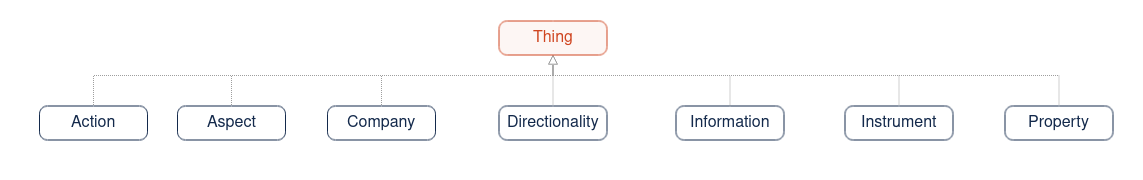
\includegraphics{/home/violetboy/media/partition2/sync/iit-codiing/CS-6852-Ontology-elective/CS-6852-Ontology/Assignment 1/image-20241019132115446.png}

\begin{enumerate}
\def\labelenumi{\arabic{enumi}.}
\item
  Information

  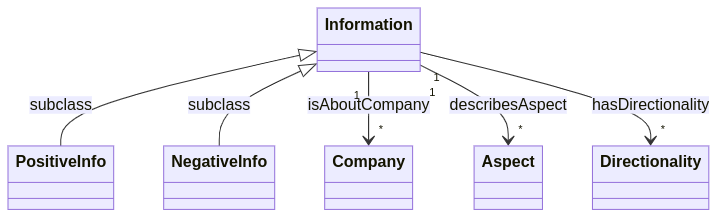
\includegraphics[width=7.46875in,height=\textheight]{17293660394468.png}
\item
  \textbf{Companies and their financial instruments}: Ontology model has
  to capture information about various companies and the financial
  instruments they issue (restricted to Bond and Stocks).

  \begin{itemize}
  \item
    Company issues Stocks and Bonds, and based on the available
    information, we have to classify the company into Positive and
    Negative sub-classes
  \end{itemize}

  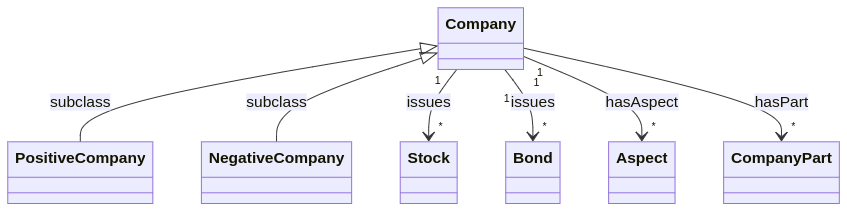
\includegraphics[width=8.82292in,height=\textheight]{17293660394659.png}

  Sample Class Structure of Instruments

  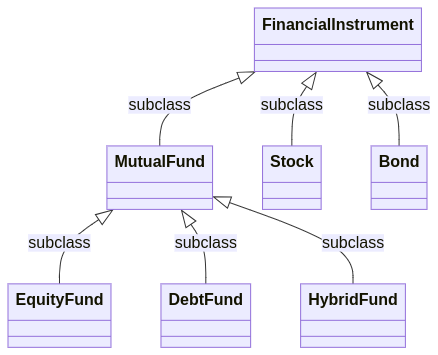
\includegraphics[width=4.5625in,height=\textheight]{172936603947810.png}
\item
  \textbf{Aspects of a company}:

  \begin{enumerate}
  \def\labelenumii{\arabic{enumii}.}
  \item
    Key attributes or aspects of company that are important to retail
    investors (e.g., stock performance, market share, earnings, or
    corporate governance).

    \begin{itemize}
    \item
      Here, the aspect can be a positive aspect (e.g., \texttt{profit},
      \texttt{share\ price}, \texttt{stores}) or a negative aspect
      (e.g., \texttt{debt}, \texttt{loss})
    \item
      Company Parts like \texttt{branches}, \texttt{stores}, etc. are
      under Positive aspects
    \end{itemize}
  \end{enumerate}

  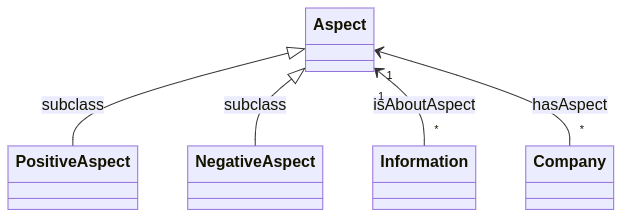
\includegraphics[width=6.46875in,height=\textheight]{172936603948911.png}
\item
  \textbf{Actions and Properties}

  \begin{itemize}
  \item
    Properties are mostly adjectives (like \texttt{lower},
    \texttt{better}, etc.) present in the information triplet that
    describe the aspect of the company and give the directionality of
    that aspect

    \begin{itemize}
    \item
      \textbf{Decreasing \& Increasing Property}

      \begin{itemize}
      \item
        Decreasing property (e.g., \texttt{lower}, \texttt{reduction})
        when combined with positive aspects (e.g., \texttt{profit},
        \texttt{margin}) will give a negative label to information
      \item
        But when combined with negative aspects (e.g., \texttt{loss},
        \texttt{margin}), it will give a positive label to information
      \item
        Similar argument can be made for Increasing property
      \end{itemize}
    \item
      \textbf{Negative and Positive Property}

      \begin{itemize}
      \item
        These are properties which inherently carry negative or positive
        sentiments irrespective of the aspect they are tied to,
      \item
        e.g., (\texttt{underperforming}, \texttt{loss-making},
        \texttt{bankrupt}, etc.) for Negative Property
      \item
        e.g., (\texttt{robust}, \texttt{successful}, etc.) for Positive
        Property
      \end{itemize}
    \end{itemize}

    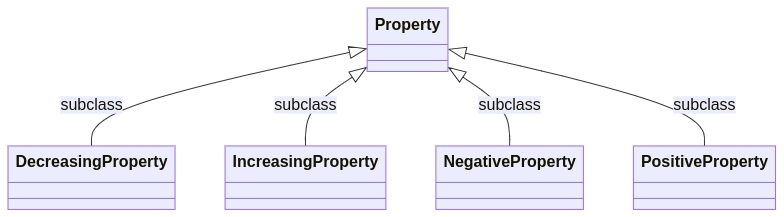
\includegraphics[width=8.15625in,height=\textheight]{172936603949912.png}
  \item
    A similar argument can be made for actions, except that actions are
    generally verbs (like \textbf{creates} jobs, \textbf{closed} stores,
    etc.)

    \begin{itemize}
    \item
      \texttt{achieves}, \texttt{declines} - examples of Negative
      Actions
    \item
      \texttt{struggles}, \texttt{loses} - examples of Positive Actions
    \item
      \texttt{reports} profit, \texttt{reports} loss, etc. - are
      examples of Increasing or Decreasing Actions that can convey
      sentiment based on the aspect they are tied to
    \end{itemize}

    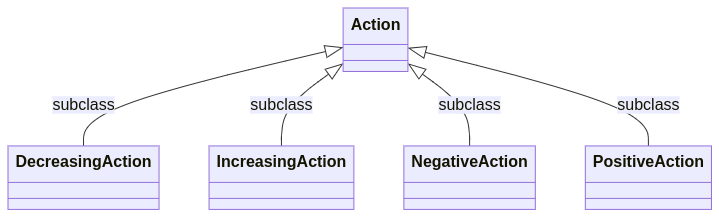
\includegraphics[width=7.48958in,height=\textheight]{172936603950813.png}
  \end{itemize}
\item
  \textbf{Directionality of the information}: Whether a change in a
  specific aspect or an event related to a company is viewed positively
  or negatively.

  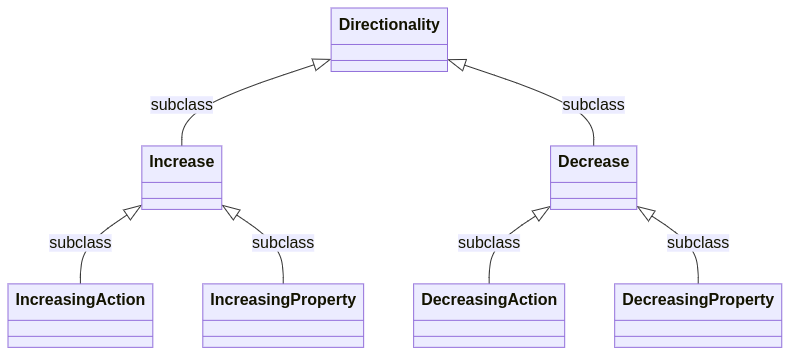
\includegraphics[width=8.21875in,height=\textheight]{172936603951914.png}

  \hfill\break
\item
  \textbf{Classification rules}: Rules that define how the combination
  of company name, aspect, and directionality translates into a Positive
  or Negative classification for an instrument.
\end{enumerate}

\subsection{Task - 2}\label{task---2}

\subsubsection{\texorpdfstring{DL ontology (TBox)
}{DL ontology (TBox) }}\label{dl-ontology-tbox}

\paragraph{Class Definition for
Instruments}\label{class-definition-for-instruments}

\textbf{Class:} \emph{Bond}

\begin{quote}
Bond \(\sqsubseteq\) Instrument\\
Bond \(\sqsubseteq\) \(\leq 1\) issuedBy.Company
\end{quote}

\textbf{Class:} \emph{Stock}

\begin{quote}
Stock \(\sqsubseteq\) Instrument\\
Stock \(\sqsubseteq\) \(\leq 1\) issuedBy.Company
\end{quote}

\textbf{Class:} \emph{AtomicInstrument}

\begin{quote}
AtomicInstrument \(\equiv\) Bond \(\sqcup\) Stock
\end{quote}

\textbf{Class:} \emph{MutualFund}

\begin{quote}
MutualFund \(\sqsubseteq\) Instrument
\end{quote}

\textbf{Class:} \emph{DebtFund}

\begin{quote}
DebtFund \(\equiv\) MutualFund \(\sqcap\) \(\forall\) hasInstrument.Bond
\end{quote}

\textbf{Class:} \emph{EquityFund}

\begin{quote}
EquityFund \(\equiv\) MutualFund \(\sqcap\) \(\forall\)
hasInstrument.Stock
\end{quote}

\begin{center}\rule{0.5\linewidth}{0.5pt}\end{center}

\textbf{Class:} \emph{Decrease}

\begin{quote}
Decrease \(\sqsubseteq\) Directionality
\end{quote}

\textbf{Class:} \emph{DecreasingAction}

\begin{quote}
DecreasingAction \(\sqsubseteq\) Action\\
DecreasingAction \(\sqsubseteq\) Decrease
\end{quote}

\textbf{Class:} \emph{DecreasingProperty}

\begin{quote}
DecreasingProperty \(\sqsubseteq\) Decrease\\
DecreasingProperty \(\sqsubseteq\) Property
\end{quote}

\textbf{Class:} \emph{Increase}

\begin{quote}
Increase \(\sqsubseteq\) Directionality
\end{quote}

\textbf{Class:} \emph{IncreasingAction}

\begin{quote}
IncreasingAction \(\sqsubseteq\) Action\\
IncreasingAction \(\sqsubseteq\) Increase
\end{quote}

\textbf{Class:} \emph{IncreasingProperty}

\begin{quote}
IncreasingProperty \(\sqsubseteq\) Increase\\
IncreasingProperty \(\sqsubseteq\) Property
\end{quote}

\begin{center}\rule{0.5\linewidth}{0.5pt}\end{center}

\textbf{Class:} \emph{NegativeAction}

\begin{quote}
NegativeAction \(\sqsubseteq\) Action\\
NegativeAction \(\sqsubseteq\) Negative
\end{quote}

\textbf{Class:} \emph{NegativeAspect}

\begin{quote}
NegativeAspect \(\sqsubseteq\) Aspect
\end{quote}

\textbf{Class:} \emph{NegativeProperty}

\begin{quote}
NegativeProperty \(\sqsubseteq\) Negative\\
NegativeProperty \(\sqsubseteq\) Property
\end{quote}

\begin{center}\rule{0.5\linewidth}{0.5pt}\end{center}

\textbf{Class:} \emph{PositiveAction}

\begin{quote}
PositiveAction \(\sqsubseteq\) Action\\
PositiveAction \(\sqsubseteq\) Positive
\end{quote}

\textbf{Class:} \emph{PositiveAspect}

\begin{quote}
PositiveAspect \(\sqsubseteq\) Aspect
\end{quote}

\textbf{Class:} \emph{PositiveProperty}

\begin{quote}
PositiveProperty \(\sqsubseteq\) Positive\\
PositiveProperty \(\sqsubseteq\) Property
\end{quote}

\begin{center}\rule{0.5\linewidth}{0.5pt}\end{center}

\textbf{Class:} \emph{NegativeInfo}

\begin{quote}
NegativeInfo \(\equiv\) (\(\exists\) describesAspect.Decrease \(\sqcap\)
\(\exists\) isAboutAspect.PositiveAspect) \(\sqcup\) (\(\exists\)
describesAspect.Increase \(\sqcap\) \(\exists\)
isAboutAspect.NegativeAspect) \(\sqcup\) (\(\exists\)
describesAspect.NegativeAction) \(\sqcup\) (\(\exists\)
describesAspect.NegativeProperty)
\end{quote}

\textbf{Class:} \emph{NegativeCompany}

\begin{quote}
NegativeCompany \(\equiv\) \(\exists\)
(isAboutCompany)\(^{-}\).NegativeInfo
\end{quote}

\textbf{Class:} \emph{NegativeStock}

\begin{quote}
NegativeStock \(\equiv\) \(\exists\) issuedBy.NegativeCompany
\end{quote}

\textbf{Class:} \emph{NegativeInstrument}

\begin{quote}
NegativeInstrument \(\equiv\) AtomicInstrument \(\sqcap\) \(\exists\)
issuedBy.NegativeCompany
\end{quote}

\textbf{Class:} \emph{NegativeMutualFund}

\begin{quote}
NegativeMutualFund \(\equiv\) \(\exists\)
hasInstrument.NegativeInstrument
\end{quote}

\begin{center}\rule{0.5\linewidth}{0.5pt}\end{center}

\textbf{Class:} \emph{PositiveInfo}

\begin{quote}
PositiveInfo \(\equiv\) (\(\exists\) describesAspect.Decrease \(\sqcap\)
\(\exists\) isAboutAspect.NegativeAspect) \(\sqcup\) (\(\exists\)
describesAspect.Increase \(\sqcap\) \(\exists\)
isAboutAspect.PositiveAspect) \(\sqcup\) (\(\exists\)
describesAspect.PositiveAction) \(\sqcup\) (\(\exists\)
describesAspect.PositiveProperty)
\end{quote}

\textbf{Class:} \emph{PositiveCompany}

\begin{quote}
PositiveCompany \(\equiv\) \(\exists\)
(isAboutCompany)\(^{-1}\).PositiveInfo
\end{quote}

\textbf{Class:} \emph{PositiveInstrument}

\begin{quote}
PositiveInstrument \(\equiv\) \(\exists\) issuedBy.PositiveCompany
\end{quote}

\textbf{Class:} \emph{PositiveMutualFund}

\begin{quote}
PositiveMutualFund \(\equiv\) \(\exists\)
hasInstrument.PositiveInstrument
\end{quote}

\textbf{Class:} \emph{PositiveStock}

\begin{quote}
PositiveStock \(\equiv\) \(\exists\) issuedBy.PositiveCompany
\end{quote}

\subsection{\texorpdfstring{Task 3 }{Task 3 }}\label{task-3}

\subsubsection{Design Choices for the Financial Instrument
Ontology}\label{design-choices-for-the-financial-instrument-ontology}

\begin{itemize}
\item
  Consider the below class diagram where black lines indicate the
  subclass relationship.

  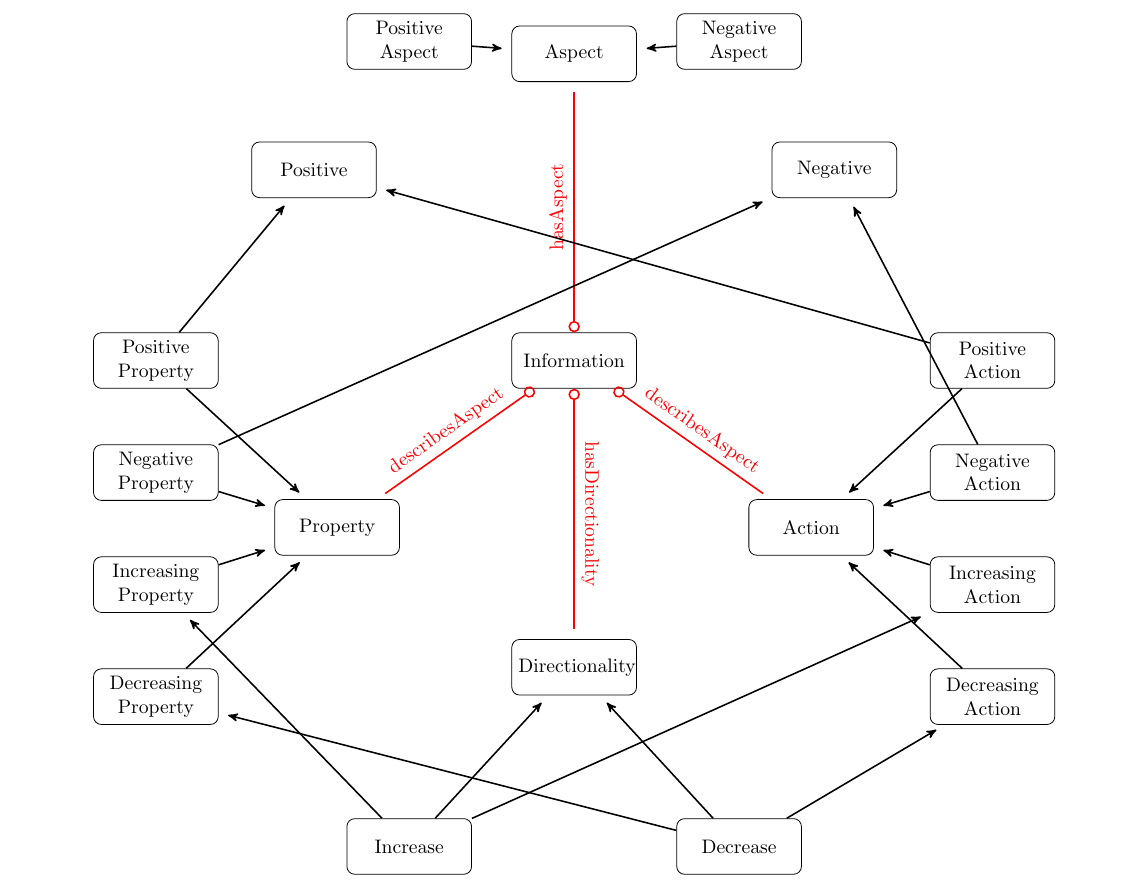
\includegraphics{/home/violetboy/media/partition2/sync/iit-codiing/CS-6852-Ontology-elective/CS-6852-Ontology/Assignment 1/image-20241019232043295.png}

  \begin{itemize}
  \item
    The core idea is to classify the aspect of the company and the
    directionality of the aspect into separate classes for easy
    modelling.
  \item
    Classifying aspect into verb and adjective enables to model words
    directly without using any external lexical processing.
  \item
    Separating directional words into aspect dependent and aspect
    independent enables easy definition of general class axioms such as

    \begin{quote}
    Decrease \(\sqcap\) NegativeAspect \(\sqsubseteq\) Positive\\
    Decrease \(\sqcap\) PositiveAspect \(\sqsubseteq\) Negative\\
    Increase \(\sqcap\) NegativeAspect \(\sqsubseteq\) Negative\\
    Increase \(\sqcap\) PositiveAspect \(\sqsubseteq\) Positive
    \end{quote}
  \end{itemize}
\end{itemize}

\subsubsection{Motivating Situations and
Examples}\label{motivating-situations-and-examples}

\subparagraph{Example 1: Stock Sentiment
Analysis}\label{example-1-stock-sentiment-analysis}

\begin{itemize}
\item
  Consider a scenario where a retail investor wants to assess the
  sentiment of a stock (say, "StockA") issued by "CompanyA". The
  investor checks recent news that "CompanyA\textquotesingle s earnings
  increased." This information would be represented in the ontology as:

  \begin{itemize}
  \item
    \texttt{Information\ isAbout\ CompanyA}
  \item
    \texttt{Information\ hasAspect\ earnings}
  \item
    \texttt{earnings} is an instance of \texttt{Class:PositiveAspect}
  \item
    \texttt{increased} is an instance of \texttt{Class:Increase}
  \item
    \texttt{PositiveAspect} \(\sqcap\) \texttt{Increase} ⊑
    \texttt{Positive}
  \item
    \(\therefore\) we can infer Information is \texttt{Positive} and
    associated company stock is also as \texttt{PositiveCompany}
  \end{itemize}
\end{itemize}

The combination of the company and the positive aspect would lead to the
classification of "StockA" as having positive sentiment.

\subparagraph{Example 2: Bond Issuance}\label{example-2-bond-issuance}

\begin{itemize}
\item
  A bond instrument "BondA" issued by "CompanyB" might be under
  consideration by a retail investor. The ontology models this as:

  \begin{itemize}
  \item
    \texttt{BondA\ issuedBy\ CompanyB}
  \end{itemize}
\end{itemize}

Additionally, if the investor finds out that "CompanyB's debt
increased," it could be represented as:

\begin{itemize}
\item
  \texttt{CompanyB\ hasAspect\ Debt\ and\ hasDirectionality\ Increase}
\item
  \texttt{Debt\ and\ Increase\ is\ a\ \ NegativeAspect}
\end{itemize}

This negative sentiment might cause the investor to avoid "BondA."

\subsubsection{Design Trade-offs and
Justifications}\label{design-trade-offs-and-justifications}

\begin{enumerate}
\def\labelenumi{\arabic{enumi}.}
\item
  \textbf{Simplified Representation for Retail Investors}:

  \begin{itemize}
  \item
    The ontology is aiming for simplicity and direct mappings of company
    aspects to instrument sentiment. This focus ensures clarity without
    the complexity of deeper financial models.
  \end{itemize}
\item
  \textbf{Triplet-based Reasoning}:

  \begin{itemize}
  \item
    The decision to model sentiment using triplets (Company, Aspect,
    Directionality) allows for a scalable and flexible approach. This
    structure easily accommodates the dynamic nature of market
    information and sentiment shifts.
  \end{itemize}
\item
  \textbf{Explicit Positive/Negative Classification}:

  \begin{itemize}
  \item
    By introducing \texttt{PositiveAspect} and \texttt{NegativeAspect}
    as distinct classes, the ontology directly supports the sentiment
    classification of financial instruments. This design enables
    straightforward rule-based classification for retail investors.
  \end{itemize}
\end{enumerate}

\subsubsection{Limitations}\label{limitations}

The current design is very limited in terms of capturing general
information related to news and events of a company. This model could be
extended by:

\begin{itemize}
\item
  \textbf{Advanced reasoning}: Implementing more complex reasoning over
  multiple aspects (e.g., combining positive and negative aspects to
  assess the overall sentiment).
\item
  \textbf{Time-based reasoning}: Capturing the evolution of sentiment
  over time to support trends.
\end{itemize}

\end{document}
